\newpage
\section{Teoría de trenzas con Matlab.}
Hemos implementado bajo Matlab R2015a todos los aspectos matemáticos que desarrollamos en el capítulo \ref{ch2}. Hemos creado métodos básicos para poder trabajar correctamente con el grupo de las trenzas. Además, hemos implementado un algoritmo muy básico para ver si una trenza dada es pura o no: diremos que una trenza es pura si su permutación se corresponde con la permutación identidad. También cabe comentar que sobre trenzas cerradas hemos implementado la notación de Dowker que vimos en el capítulo \ref{ch1} sobre teoría de nudos. \\

Para recopilar todo este conjunto de herramientas que nos permiten trabajar con trenzas hemos creado \textbf{toxtren}. Se trata de un toolbox, una librería de funciones Matlab, asociado al estudio de trenzas y trenzas cerradas \cite{6}.  \\ 

Para hacer uso de toxtren, el usuario simplemente tiene que disponer de Matlab e instalar toxtren.mltbx: seleccionamos como nuevo directorio de trabajo la carpeta que contiene el archivo .mltbx, hacemos click derecho sobre él e instalamos. \\

Para realizar el control de versiones de toxtren hemos utilizado git.\\

A la hora de implementar toxtren hemos seguido un diseño orientado a objetos ya que las trenzas se pueden representar de una forma cómoda haciendo uso de objetos y clases. En concreto, hemos construido dos clases: 
\begin{itemize}
	\item Clase trenza: mediante esta clase podremos crear cualquier trenza, visualizarla en 3D, obtener los invariantes que hemos explicado en el capítulo \ref{ch2}, estudiar su trivialidad, realizar operaciones básicas con distintas trenzas....
	\item Clase trenza\_cerrada: la clase trenza\_cerrada hereda de la clase trenza pues una trenza cerrada es una trenza en la que conectamos los extremos de las cadenas. Al hacer esta unión sobre los extremos de las cadenas podemos obtener varios enlaces: si únicamente tenemos un enlace, dicha trenza cerrada será equivalente a un nudo. \\
	En dicha clase heredamos los métodos que hemos comentado para la clase trenza y además estudiamos la notación Dowker de la trenza cerrada, el polinomio de Alexander, podemos realizar los movimientos de Markov...
\end{itemize} 

Podemos ver un esquema de la herencia de las clases con sus atributos y métodos en la figura \ref{escl}.\\

Para generar la documentación de Toxtren \cite{15}, hemos creado ficheros de ayuda HTML a partir de distintos script Matlab que contienen la documentación para ambas clases y ejemplos de uso para una mejor comprensión. Además, hemos creado los ficheros info.xml y helptoc.xml para identificar los ficheros HTML en la creación del toolbox y mostrar el panel de contenido en el buscador de ayuda.\\

De este modo, podemos obtener la documentación de toxtren tras su instalación seleccionando, en el buscador de ayuda, Toxtren Toolbox, que se encontrará en la sección Supplemental Software. También podemos hacer uso de help en la ventana de comandos. 

\begin{figure}[h!]
	\centering
	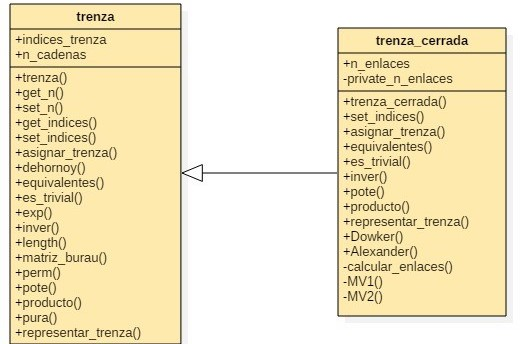
\includegraphics[width=11cm]{img/Main.jpg}
	\caption{Estructura clases}
	\label{escl} 
\end{figure}
 
\begin{figure}[h!]
	\centering
	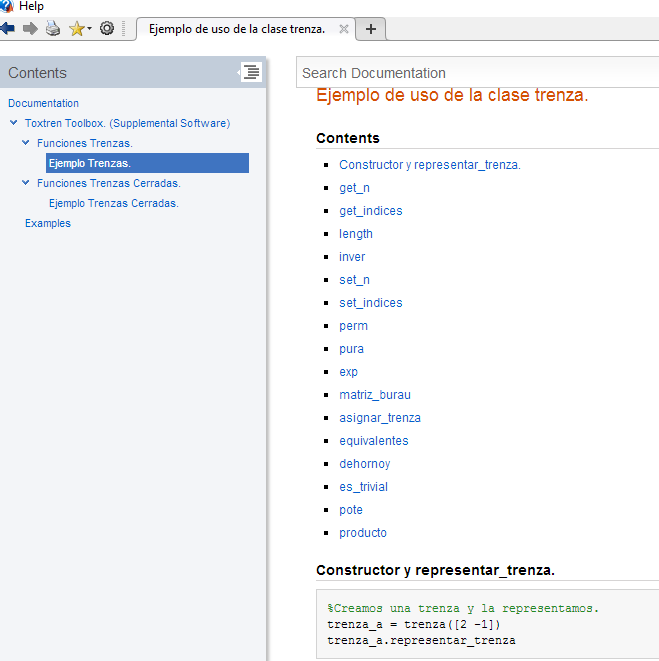
\includegraphics[width=13cm]{img/docu.png}
	\caption{Documentación Toxtren.}
	\label{docu1} 
\end{figure}